\section{Pipeline Characteristics}
\subsection*{Number of Stages}
\hspace{\parindent}The Cortex-A72 processor has a variable-length pipeline, the minimum length of which is 15 stages. This is a result of the different functional units included in the CPU, and so the maximum pipeline length can vary in other ARMv8-based processors. \cite{a72pipeline}
\subsection*{Names}
\hspace{\parindent}To simplify the the pipeline model, its stages can be divided into 5 groups and named according to the function that is performed: \cite{cortexA72manual}
\begin{itemize}
	\item \textbf{Fetch}, during cycles 1-5.
	\item \textbf{Decode}, during cycles 6-12.
	\item \textbf{Issue}, in cycle 13.
	\item \textbf{Execute}, during the following cycles, depending on the used functional unit; integer and branch operations take the shortest, at only one cycle.
	\item \textbf{Retire}, in the last cycle.
\end{itemize}
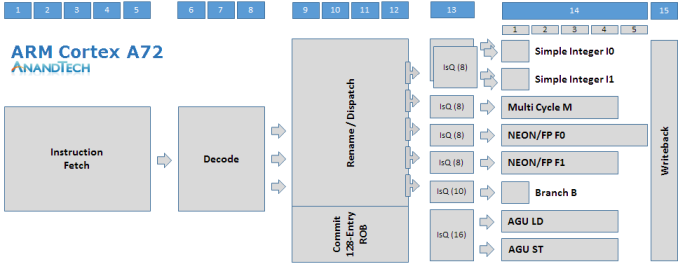
\includegraphics[width=1\linewidth]{imgs/a72pipeline.png}
\caption{The Cortex-A72 pipeline}

\section{Steps of Instruction Execution}
%TODO

\section{Performance Studies}
%TODO

